\chapter{Testovanie}

\label{kap:testovanie}

Aplikáciu sme testovali dvoma spôsobmi. Najskôr sme nappísali a spustili unit testy pomocou knižnice xUnit. Následne sme sa pozreli na ručné používanie 
samotnej aplikácie a testovanie používateľského rozhrania.

\section{Testovanie unit testami}
Unit testy sú metóda testovania softvéru, kedy je softvér rozdelený na veľa malých jednotiek (z anglického units), a každá časť je otestovaná 
samostatne \cite{unit_tests}. V našom kóde sme ako jednotky brali public metódy tried. 

Pre unit testovanie v jazyku C\# sa najčastejšie používajú riešenia MSTest, NUnit a xUnit \cite{unit_test_comparison}. Každá z nich ponúka 
všetky pre nás dôležité funkcionality, takže výber je možné spraviť podľa osobnej preferencie. Vybrali sme si knižnicu xUnit pretože nám 
najviac vyhovoval spôsob overovania výsledkov (všetky knižnice používajú triedu s názvom Assert, každá je však inako implementovaná).

Pri písaní unit testov sa najčastejšie postupuje tak, že triedam vložíme namiesto skutočných objektov sprostredkúvajúcich dáta, napríklad inštancie 
IpInfoViewerDbRepository, objekty vracajúce vymyslené, nami definované dáta. Tetno proces sa nazýva mockovanie. Mockovanie je možné vďaka použitiu návrhového 
vzoru vkladanie závislosti. Tento vzor určuje, že trieda by nemala vytvárať inštanciu inej triedy a teda byť od nej závislá, ale namiesto toho by mala len 
prijímať inštancie spĺňajúce definované rozhranie \cite{dependency_injection}. Vytváranie mockovacích objektov zabezpečjeme pomocou knižnice Moq. Tá nám šetrí 
prácu, pretože nemusíme pre každý mockup vytvárať novú triedu, ale len zadefinujeme dáta, ktoré chceme aby nám inštancia vrátila. Knižnica Moq nám 
takúto inštanciu spĺňajúcu potrebné rozhranie vytvorí \cite{moq}.

Pri písaní unit testov pomocou knižnice xUnit sa testovacie metódy označujú atribútmi \lstinline{Fact} a \lstinline{Theory}. Kým metódy s atribútom 
\lstinline{Fact} slúžia ako testy bez parametrov, metódy s atribútom \lstinline{Theory} doplnené parametrom \lstinline{InlineData} prijímajú aj parametre 
\cite{xunit_docs}.

Naším cieľom bolo vytvoriť sadu unit testov pre každú metódu z tried, ktoré sa starajú o logickú časť backendovej časti, teda \lstinline{Week}, 
\lstinline{DateTimeUtilities}, \lstinline{GeographicUtilities}, \lstinline{CountryPingInfoFacade}, \lstinline{IpAddressInfoFacade} a \lstinline{MapPointsFacade}.
Triedy \lstinline{MFileDbRepository} a \lstinline{IpInfoViewerDbRepository} úmyselne netestujeme pretože v jazyku C\# neexistuje dobrý spôsob na simuláciu 
volania SQL databázy. Taktiež nepíšeme testy na kontrolery, pretože tie v našej implementácií dáta čisto len predávajú z nižšej vrstvy, preto nie je potrebné 
ich testovať unit testami. Chyby v takomto predávaní dát by sa v každom prípade rýchlo prejavili pri používaní webovej aplikácie, čomu sa venujeme v sekcii 
\ref{test_interface}.

\section{Testovanie používateľského rozhrania}
V tejto časti otestujeme používanie aplikácie podľa scenárov definovaných v kapitole \ref{scenare}. Pre testovcie účely sme aplikáciu nasadili na adrese 
\href{https://bp.trencansky.com/}{https://bp.trencansky.com}. Podľa scenára sa po otvorení stránky zobrazí aplikácia s mapou a bodmi na nej ako vidno 
na obrázku \ref{obr:uvod_stranka}, čím je splnený bod 1. v zozname. Tiež je vidno slektor týždňov, voľba škály, a voľba zobrazených dát pre daný týždeň, čím sú 
splnené body 2, 3, a 4.   
\begin{figure}
    \centerline{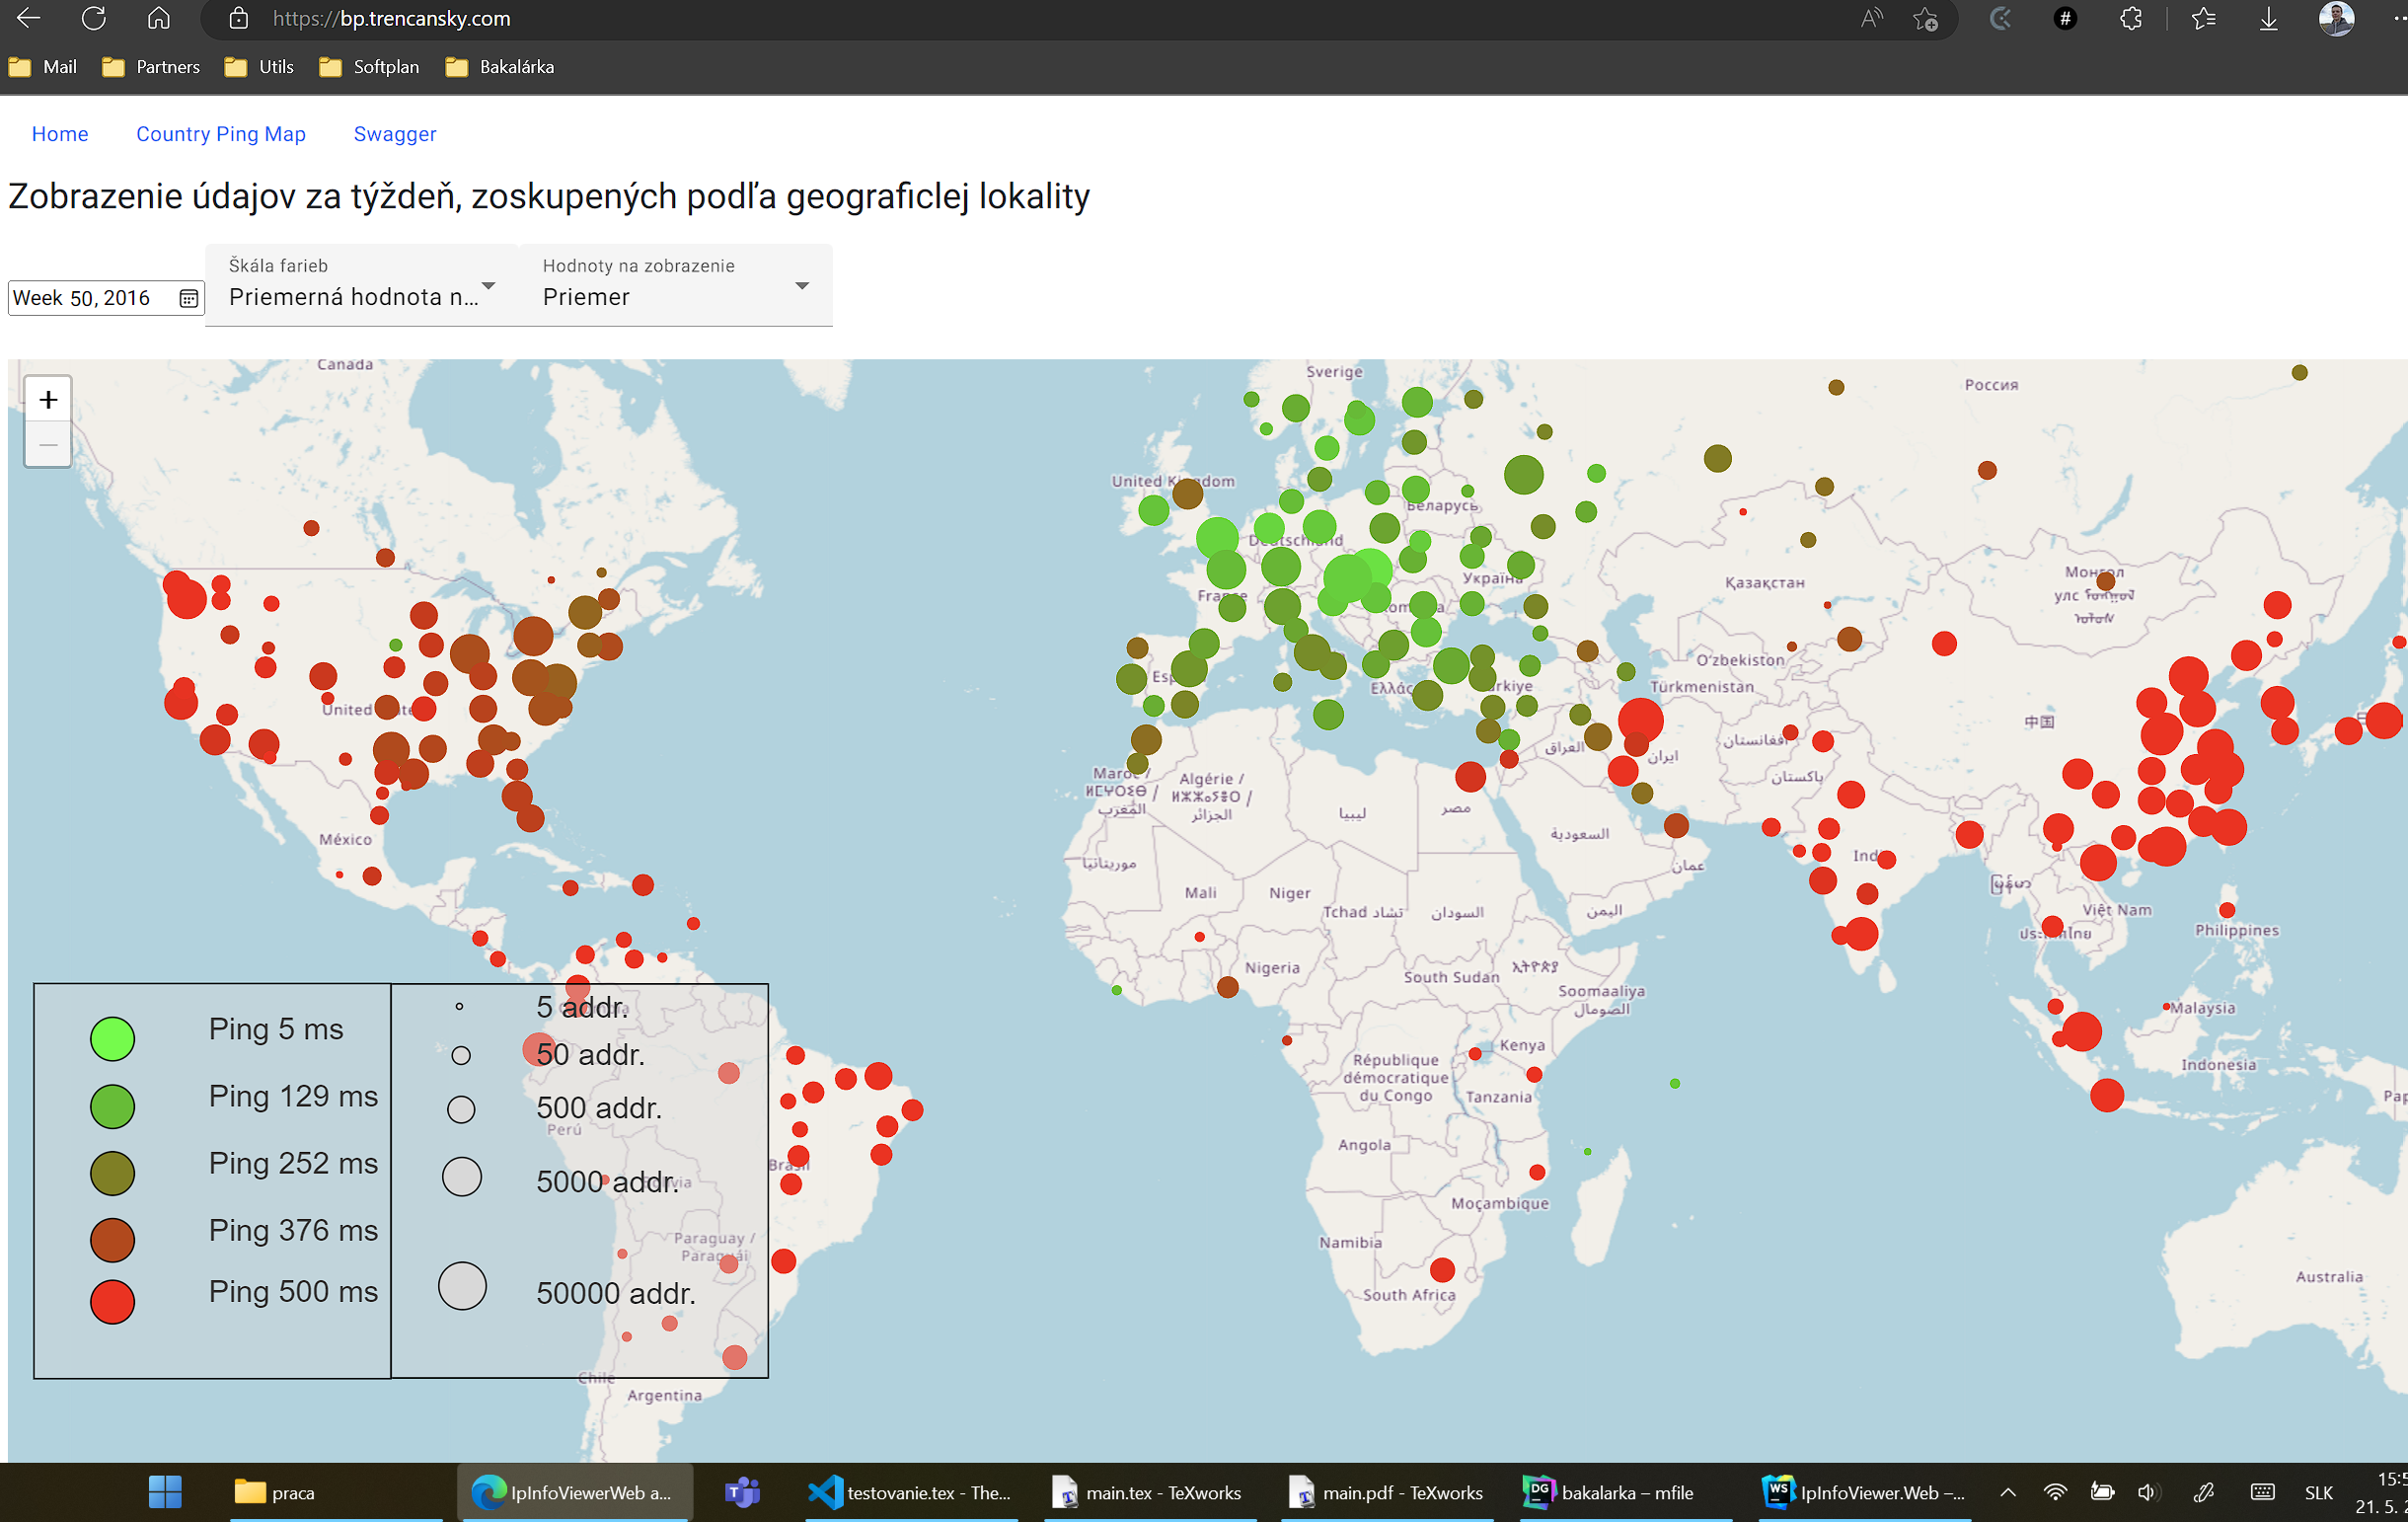
\includegraphics[width=0.8\textwidth]{images/uvodna_stranka}}
    %popis obrazku
    \caption[Úvodná stránka aplikácie]{Úvodná stránka aplikácie}
    %id obrazku, pomocou ktoreho sa budeme na obrazok odvolavat
    \label{obr:uvod_stranka}
\end{figure}
\label{test_interface}

Pokračujeme testovaním automatického prekresľovania po prepnutí selektorov. Tento test prebehne úspešne, dáta sú prekreslené po každom prepnutí selektorov.
Splnený je teda aj bod 5. Na stránke je tiež viditeľná legenda, čo spĺňa aj bod 6. Bod 7 vidíme zobrazený na obrázku \ref{obr:max_zoom}. 

Obrázok \ref{obr:country_ping_info} nám ukazuje zobrazenie mapy krajín zafarbených podľa priemernej doby odozvy, čím sa potvrdzuje bod 8 z používateľských
scenárov. Taktiež podľa bodu 9 vidíme selektory týždňov, škály a zvolených dát, ktoré tiež okamžite reagujú na zmenu, čím sa potvrdzuje bod 10. 
Bod 11 sme otestovali na väčšine krajín a vždy fungoval. Príklad môžme vidieť v obrázku \ref{obr:country_ping_tooltip}.

Keďže sme otestovali všetky scenáre bez nájdenia nedostatku, test považujeme za úspešný.

\begin{figure}
    \centerline{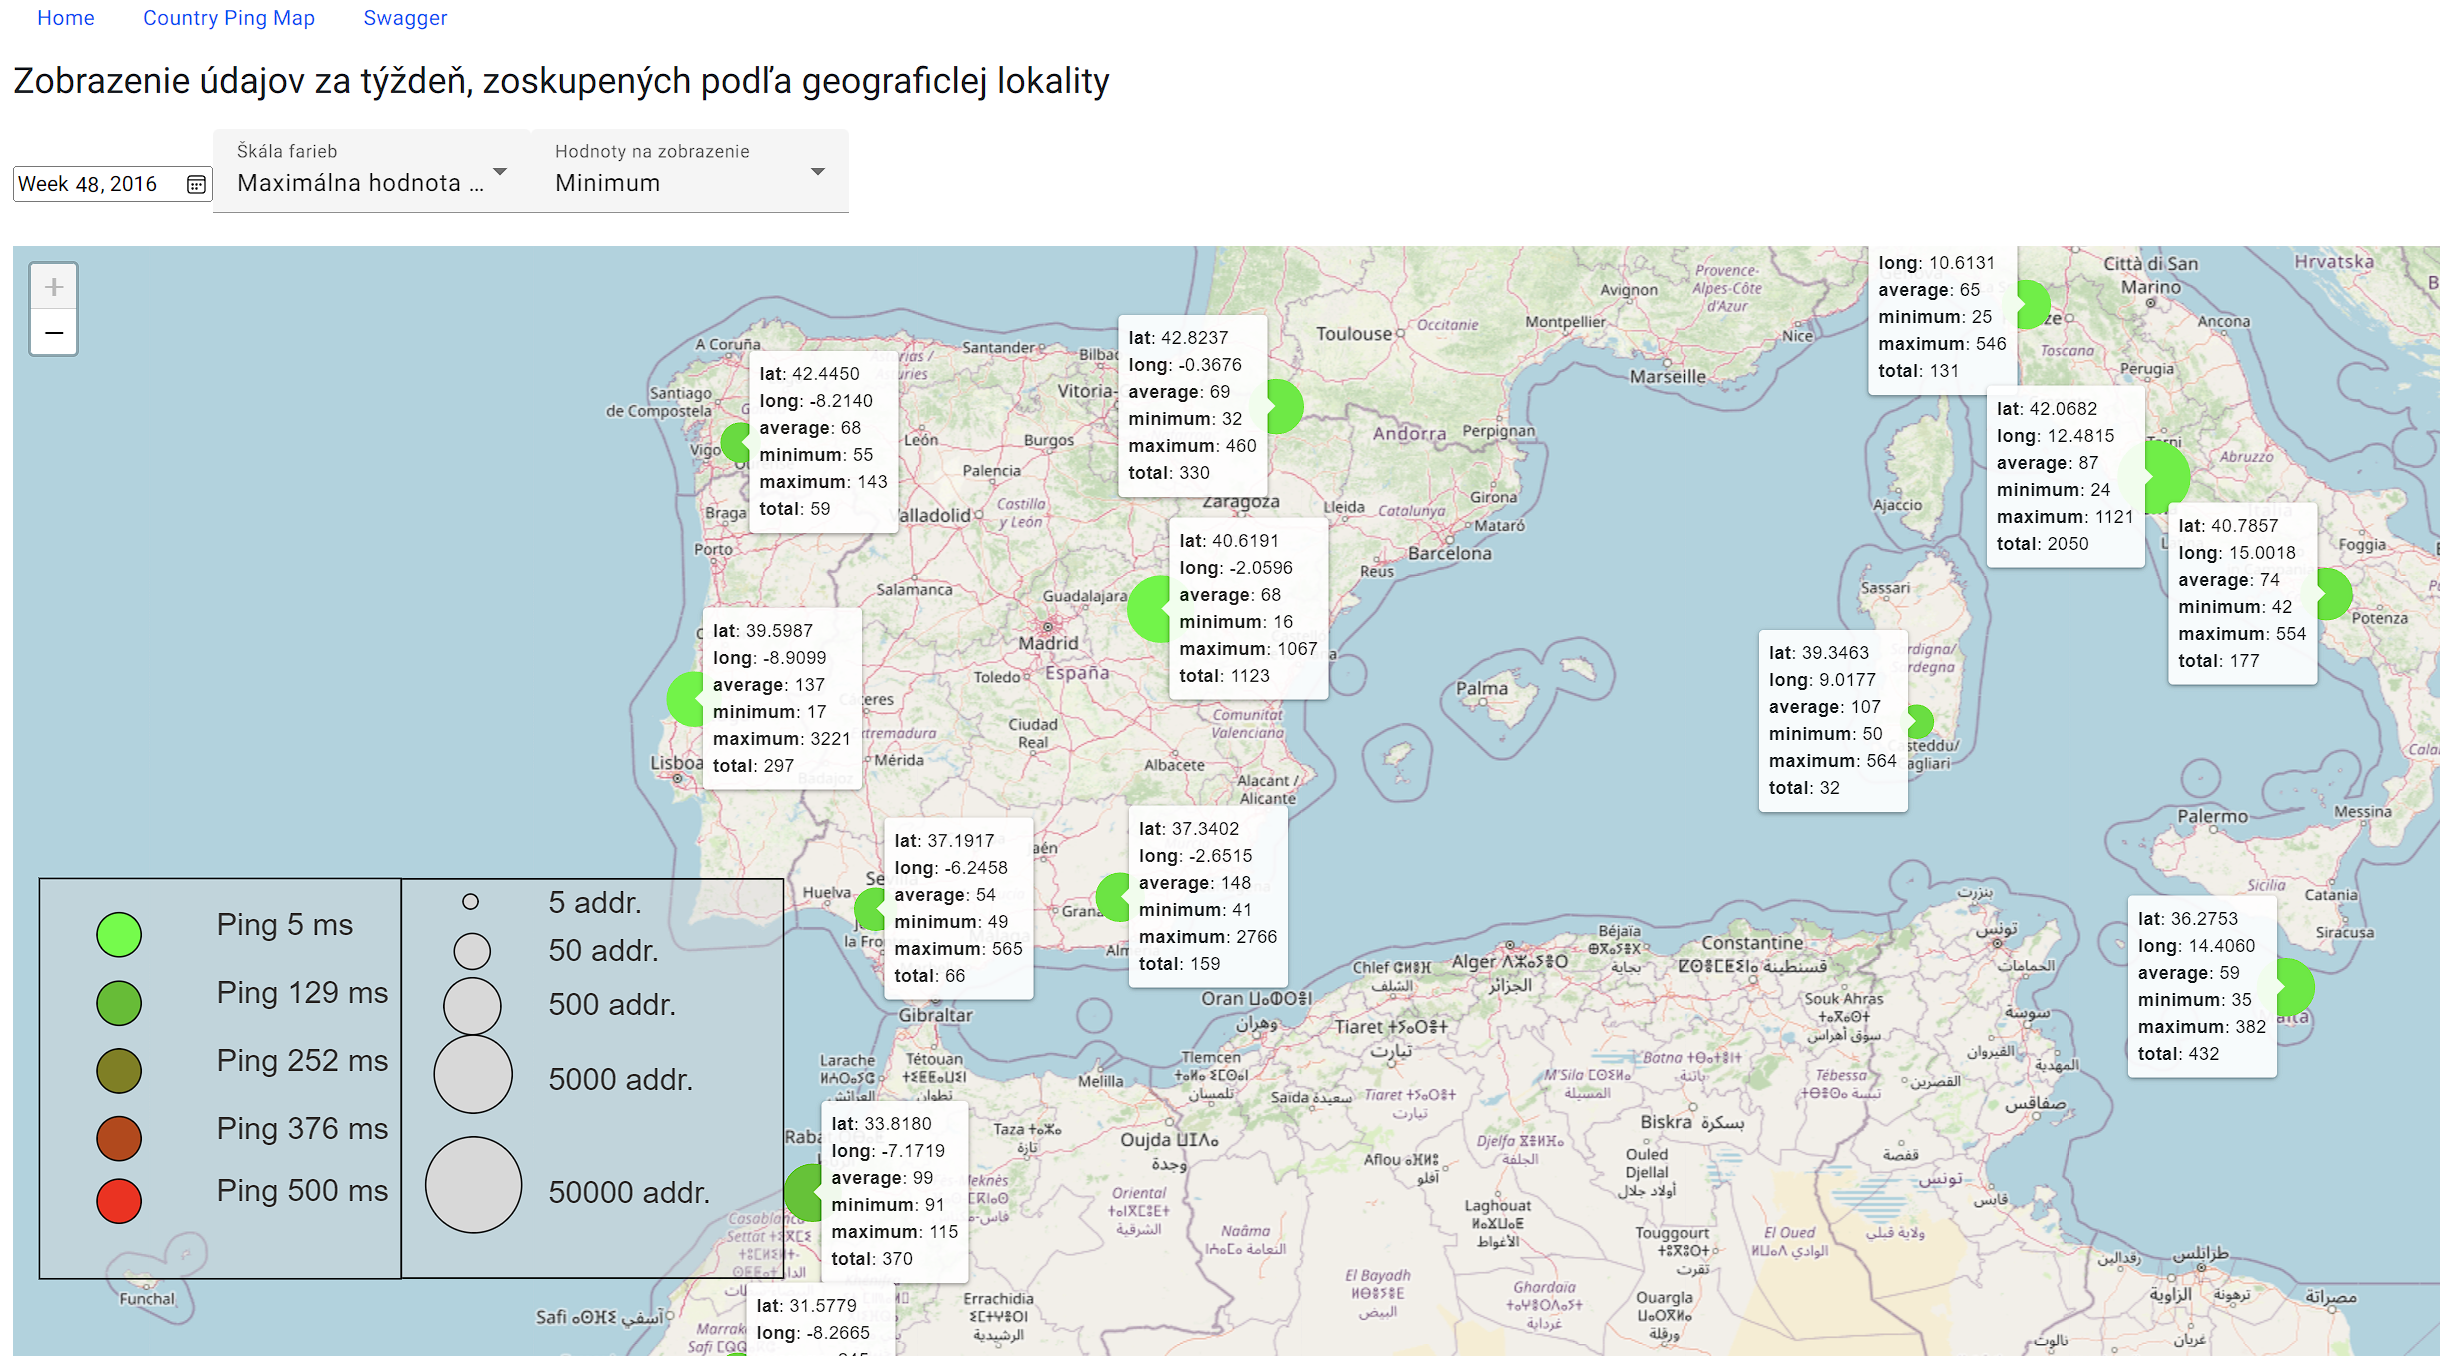
\includegraphics[width=0.8\textwidth]{images/max_zoom}}
    %popis obrazku
    \caption[Zobrazenie detailných informácií pri maximálnej úrovni priblíženia]{Zobrazenie detailných informácií pri maximálnej úrovni priblíženia}
    %id obrazku, pomocou ktoreho sa budeme na obrazok odvolavat
    \label{obr:max_zoom}
\end{figure}
\label{test_interface}



\begin{figure}
    \centerline{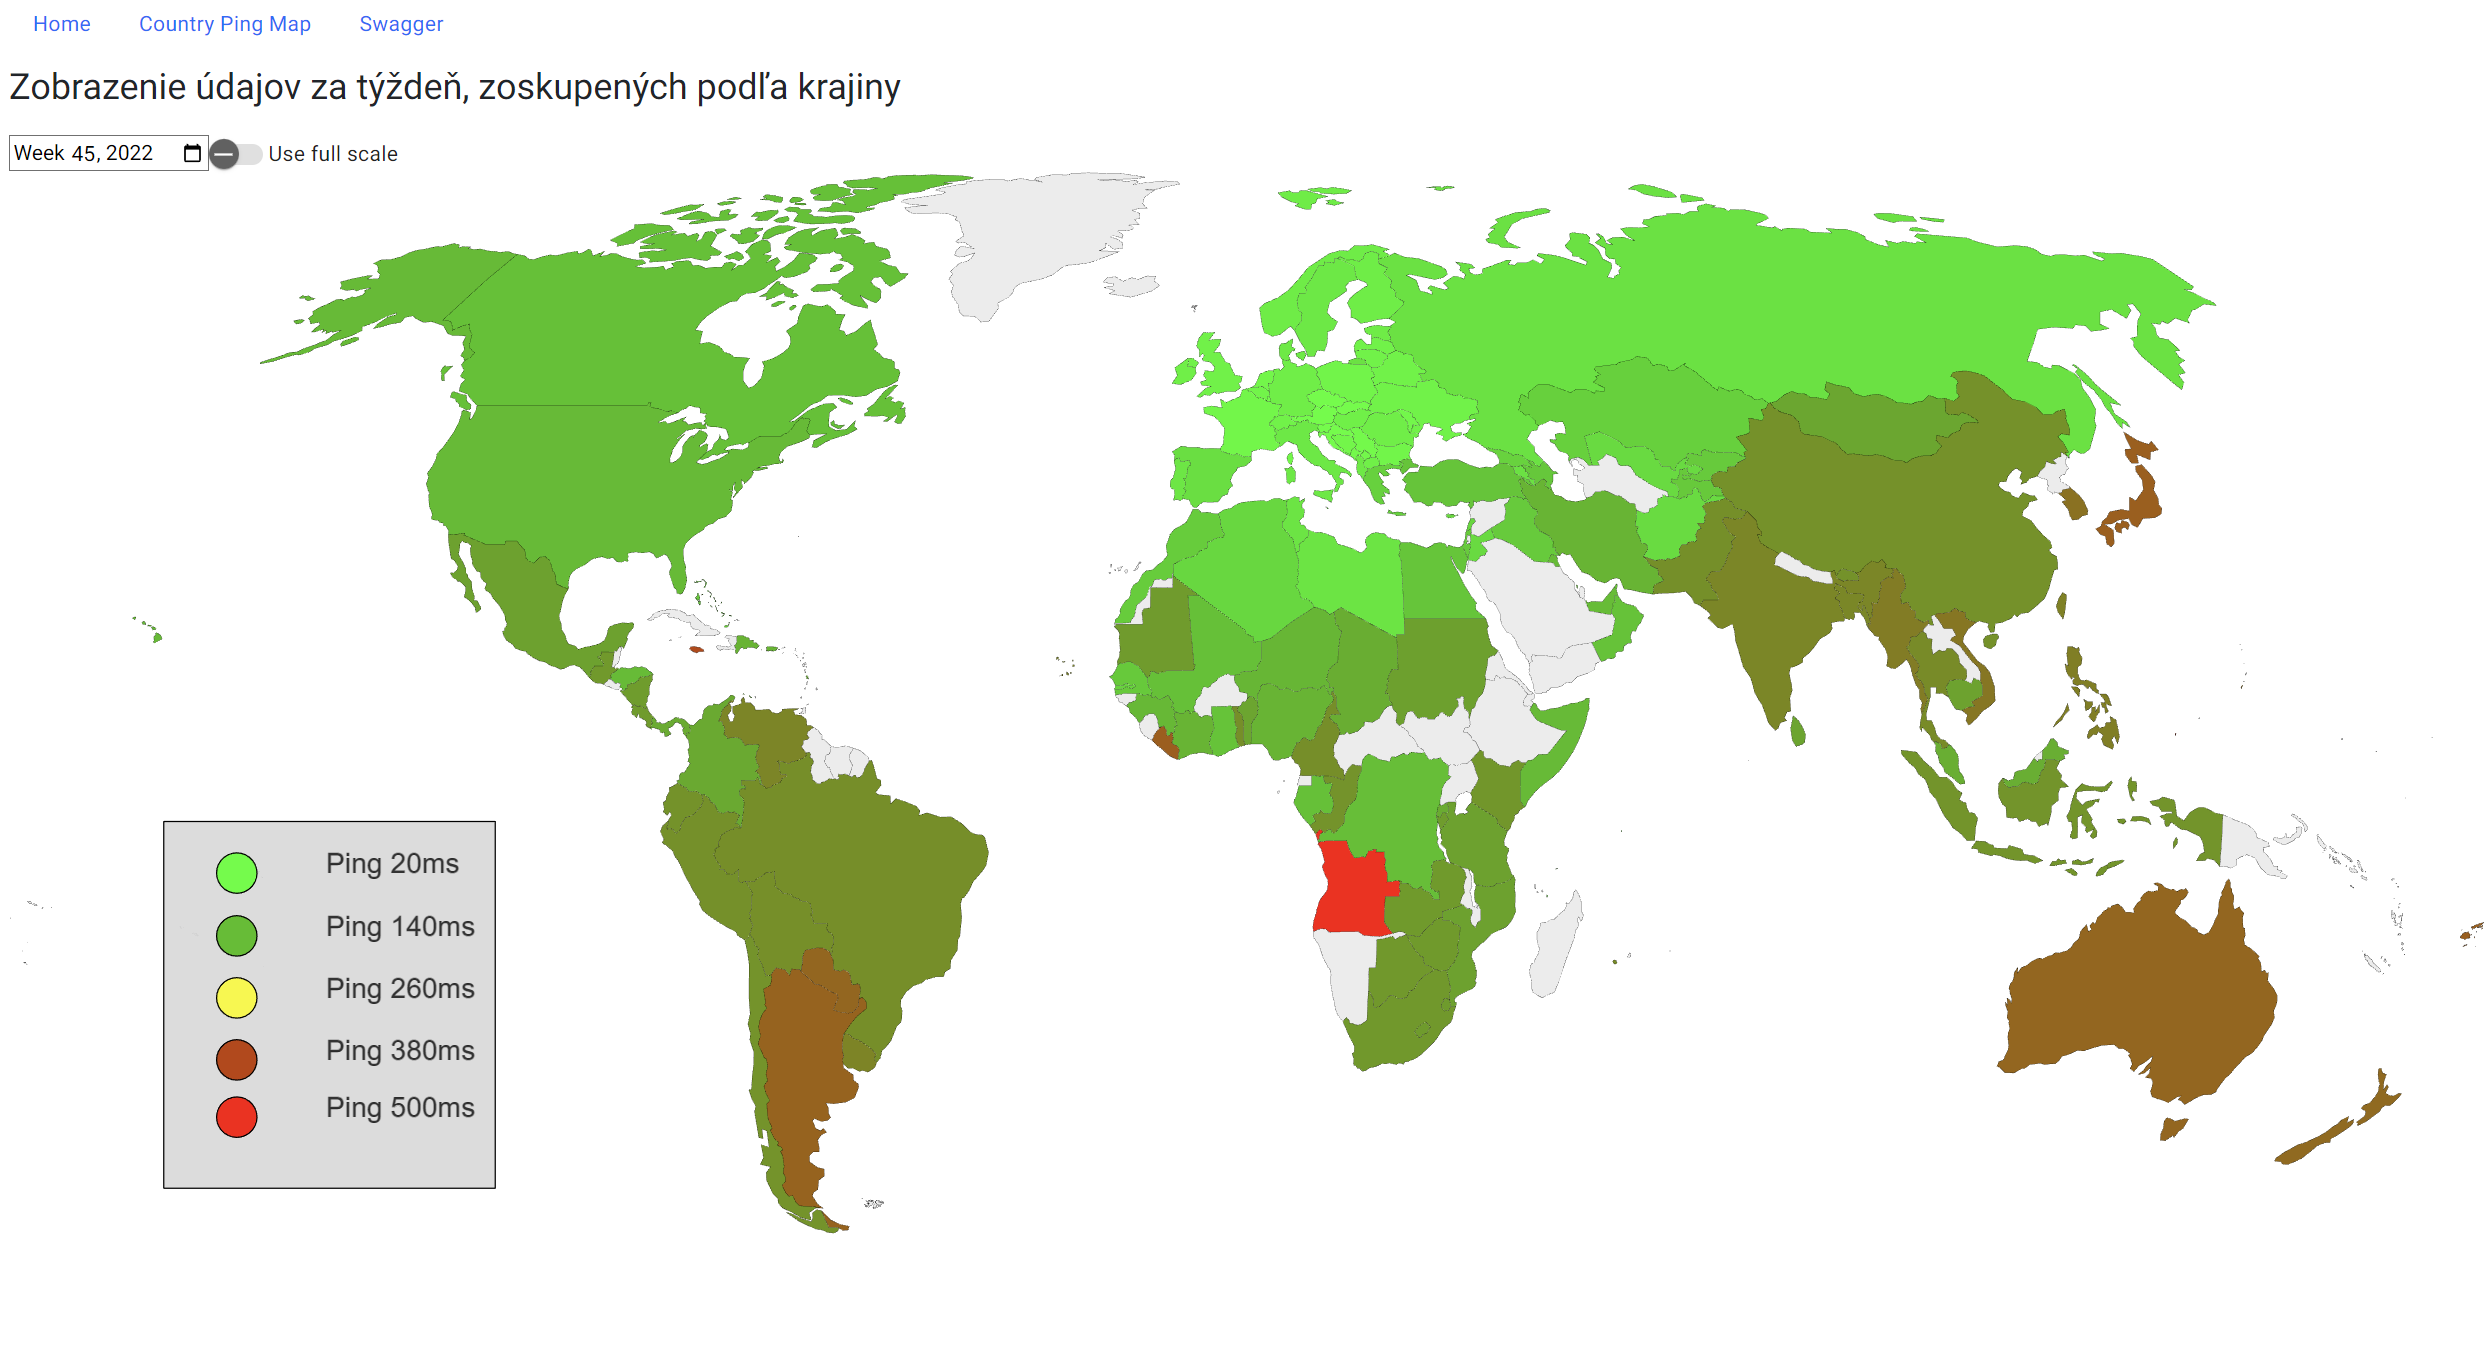
\includegraphics[width=0.8\textwidth]{images/country-ping-info}}
    %popis obrazku
    \caption[Mapa krajín zafarbených podľa priemernej doby odozvy]{Mapa krajín zafarbených podľa priemernej doby odozvy. Na podstránke je vidno hlavné menu, 
    taktiež pod ním selektor týždňov, selektor škály a samotnú mapu s legendou.}
    %id obrazku, pomocou ktoreho sa budeme na obrazok odvolavat
    \label{obr:country_ping_info}
\end{figure}


\begin{figure}
    \centerline{
\includegraphics[width=0.8\textwidth]{images/country_ping_tooltip}}
    %popis obrazku
    \caption[Zobrazenie vyskakovacieho okna pri podržaní myšou nad krajinou]{Zobrazenie vyskakovacieho okna pri podržaní myšou nad krajinou. Názov krajiny dopĺňa
    počet IP adries, maximálna, minimálna a priemerná doba odozvy.}
    %id obrazku, pomocou ktoreho sa budeme na obrazok odvolavat
    \label{obr:country_ping_tooltip}
\end{figure}